\RequirePackage{fix-cm}
\documentclass[smallextended]{svjour3}    
\smartqed  % flush right qed marks, e.g. at end of proof
\usepackage{graphicx}
\usepackage{epigraph}
\usepackage{amsthm}
\usepackage[version=4]{mhchem}

\usepackage{xcolor}
\usepackage{wrapfig}  % Add this in the preamble if not already included
\usepackage{relsize}    % For \smaller
\usepackage{url}        % For \url
\usepackage{amsmath}
\graphicspath{{pix/}}   % Root directory of the pictures 
\usepackage{graphicx}
\usepackage{amsmath}

\usepackage[font=small]{caption}
\usepackage{ragged2e} % for \raggedright alignment
\usepackage{float} 
\usepackage{pgfplots}
\usepackage[version=4]{mhchem}

\usepackage{amsmath}
\usepackage{tikz}
\newtheorem{definition}
\begin{document}

\title{Nuclear energy fundamentals}

\author{Byron J. Encinas Velázquez \and A. Balam Sotelo Cortéz
}

\institute{F. Author \at
              first address \\
              Tel.: +123-45-678910\\
              Fax: +123-45-678910\\
              \email{fauthor@example.com}           %  \\
%             \emph{Present address:} of F. Author  %  if needed
           \and
           S. Author \at
              second address
}

\date{Received: date / Accepted: date}
% The correct dates will be entered by the editor

\maketitle

\begin{abstract}
The field has been evolving at an incredible pace, with the clean energy movement in support of nuclear energy and the increased presence of start-ups and international fusion projects like ITER, W7-X, etc. The current state of science and technology allows for the assessment of key problems that will eventually make a reality of the idea that fusion and fission power plants can be the primary sources of energy. There are lots of resources in introductory plasma and nuclear physics available online, yet their advantage goes harder for the writer, who is actively studying during the writing process than for any young PhD starting his research.  We aim to develop a basic theory on fission nuclear reactor physics as well as plasma and tokamak/stellarator theory. Special attention will be given to difficulties with the theory, safety issues, and historical development for both cases. 

\end{abstract}

\newpage

\section{Historical Background}

- Eddington on the energy production in stars

- Hydrogen bomb

- 1950 Toroidal magnetic confinement (stellerator and tokamak)


The following quote comes from Homi J. Bhabha (1955).

\begin{quote}
    Its well known that atomic energy can be obtained by a fusion process as in the H bomb[...]. The technical problems are formidable, but one shuld remember that its not yet 15 years since atomic energy was released in an atomic pile for the first time by Fermi. I venture to predict that a method will be found for liberating fusion energy in a controlled manner within the next two decades. When that happens the energy problems of the world will truly have been solved forever for the fuel will be as plentiful as the heavy hydrogen in the oceans.
\end{quote}

Spitzer stellarator

Tokamak studies in rusia

ITER, WX-7

There is also inertial confinemment, z-pinch and theta-pinch

\section{Plasma physics basics}

\subsection{Definition of plasma}

\begin{definition}
\textit{A plasma is a quasineutral gas of charged and neutral particles that exhibits collective behavior}
\end{definition}

Collective behavior refers to the long-range coulombic interactions driving the motion of the particles forming the plasma, causing it to depend not on local conditions but on the properties of the whole system. 

\subsection{Debye shielding}

Quasineutrality arises as a consequence of the distribution and interaction of charged particles in the plasma. At low temperatures, thermal motion becomes negligible, so ions and positively charged particles get surrounded by a cloud of electrons completely shielding the potential, so no electric field will be perceived in the exterior of the electron cloud. With temperature $T$ the cloud expands to the edge of the ion to a distance where the potential matches the thermal energy partially shielding the charge, causing a weak electric field in the plasma.

The scale of the cloud is of the order,

\begin{equation}
    \lambda_D = \left( \frac{k_B T}{4\pi n e^2}\right)^{1/2}
\end{equation}

so that the potential decreases with radius as,
\begin{equation}
\phi(r) = \phi_0 e^{-r/\lambda_D}
\end{equation}

This concept is valid for plasmas with numerous particles in the system. The order of magnitude of particles in the plasma will prove insufficient to  refer to it as a plasma. This density of particles has to be a lot greater that the order of unity in a volume of radius debye length.

\subsection{Plasma frequency}

A neutral plasma in thermal equilibrium, ions (given their significant mass in comparison with electrons) are considered static and uniformly distributed. Still, a large enough group of electrons in motion can perturb the ions causing by coulomb interaction a pull back, as a restoring force. This yield oscillations in the plasma density.
The oscillation angular frequency of the plasma is
\begin{equation}
    \omega_e = \left( \frac{n_e e^2}{\epsilon_0 m_e}\right)^{1/2}
\end{equation}
and similarly for ions,

\begin{equation}
    \omega_i = \left( \frac{n_i q_i^2}{\epsilon_0 m_i}\right)^{1/2}
\end{equation}

There is a different definition for cases when the oscillation wavelength is larger than the debye length. So far the order of magnitude is $\omega_e = 56.4 n_e^{1/2} s^{-1}$ for a specific species density.

\subsection{Single particle motion}

A charged particle moving in an electromagnetic field is subject to the **Lorentz force**, given by:

\begin{equation}
    \mathbf{F}_L = q (\mathbf{E} + \mathbf{v} \times \mathbf{B}).
\end{equation}

If the magnetic field is **uniform** and aligned with the \( z \)-axis, i.e., \( \mathbf{B} = B_z \mathbf{e}_z \), then the equation of motion simplifies to:

\begin{equation}
    m \frac{d\mathbf{v}}{dt} = q \mathbf{v} \times \mathbf{B}.
\end{equation}

This interaction causes the particle to undergo **helical motion**, where its velocity components evolve as:

\[
\mathbf{v} =
\begin{pmatrix}
v_{\perp} \cos(\omega t) \\
v_{\perp} \sin(\omega t) \\
v_{\parallel}
\end{pmatrix}.
\]

Here, \( v_{\perp} \) represents motion in the plane perpendicular to the field, while \( v_{\parallel} \) describes free movement along \( \mathbf{B} \). The **cyclotron frequency**, which determines the rate of circular motion, is:
\begin{equation}
    \omega = \frac{q B_z}{m}.
\end{equation}

The radius of this gyration, known as the \textit{Larmor radius}, is:

\begin{equation}
    r_L = \frac{v_\perp}{\omega} = \frac{m v_{\perp}}{q B_z}.
\end{equation}

This circular motion plays a crucial role in plasma physics, confinement systems, and space environments. Additionally, the charge’s tendency to drift in response to external forces leads to \textit{diamagnetic effects}, where the motion effectively opposes changes in the magnetic field. 

\subsection{Magnetic mirror}

We start talking about the first adiabatic invariant, which is of major important in the description of particles in the local magnetic fields.

\begin{equation}
    \oint p ds = \mu_m = \frac{\frac{1}{2}m\Vec{v}_\perp ^2}{B}
    \label{AdInvariant}
\end{equation}
By substituing $v_{\perp}^2 = v^2 \sin(\alpha)$ where $\alpha$ is the angle between magnetic field and velocity vector. If this is a conserved quantity (no scattering) along the motion, then its bounded by a previous value of the magnetic field and the angle $\alpha_i$ at that moment.
\begin{equation}
\frac{\sin^2(\alpha) }{B(s)}=\frac{\sin^2(\alpha_i) }{B_i} 
\end{equation}

Pitch angles evolve as $sin(\alpha(s)) = \sqrt{\frac{B(s)}{B_i}}sin(\alpha_i)$. This marks the initial pitch angle $\alpha_i$ that gets mirrored at $s$ if the inequality is not fulfilled. 
\begin{equation}
    \sin(\alpha_i) < \sqrt{B_i / B(s)}
\end{equation}

\subsection{Velocity drift}

The drift velocity of a charged particle due to an external force and magnetic field variations is given by:

\begin{itemize}
    \item \textbf{External Force Drift:}
    \[
    \mathbf{v}_F = \frac{\mathbf{F} \times \mathbf{B}}{q B^2}
    \]
    where \( q \) is the particle charge, and \( B = |\mathbf{B}| \) is the magnetic field magnitude.

    \item \textbf{Gradient-\( B \) Drift:}
    \[
    \mathbf{v}_{\nabla B} = \frac{m v_\perp^2}{2 q B^2} (\mathbf{B} \times \nabla B)
    \]
    where \( m \) is the particle mass, \( v_\perp \) is the velocity component perpendicular to \( \mathbf{B} \), and \( \nabla B \) represents the magnetic field gradient.

    \item \textbf{Curvature Drift:}
    \[
    \mathbf{v}_c = \frac{m v_\parallel^2}{q B^2} (\mathbf{B} \times \mathbf{R}_c)
    \]
    where \( v_\parallel \) is the velocity parallel to \( \mathbf{B} \), and \( \mathbf{R}_c \) is the radius of curvature of the magnetic field lines.

     \item \textbf{Diamagnetic Drift:}
    \[
    \mathbf{v}_D = \frac{\nabla P \times \mathbf{B}}{q n B^2}
    \]
    where \( P \) is the plasma pressure, and \( n \) is the particle number density. The diamagnetic drift arises due to the pressure gradient in a magnetized plasma.

\end{itemize}
\subsection{Collision vs collisionless plasma}
\subsection{MHD and stability}

Fundamental MHD equations (diff between ideal and non ideal)
Frozen-in flux in ideal MHD
types of plasma instabilities (e.g., Rayleigh-Taylor, kink, tearing mode) and their impact on confinement
magnetic reconnection instability
classical, neoclassical, and turbulent transport in plasmas
magnetic shear in plasma stability
 zonal flows in suppressing turbulence in fusion plasmas
 Alfvén waves and magnetosonic waves
 Landau damping and its role in wave-particle interactions
 main heating methods used in fusion plasmas (e.g., ohmic heating, neutral beam injection, electron and ion cyclotron resonance heating)
\newpage
\section{Thermonuclear fusion}

\subsection{Fusion reactions}

\begin{figure}
    \centering
    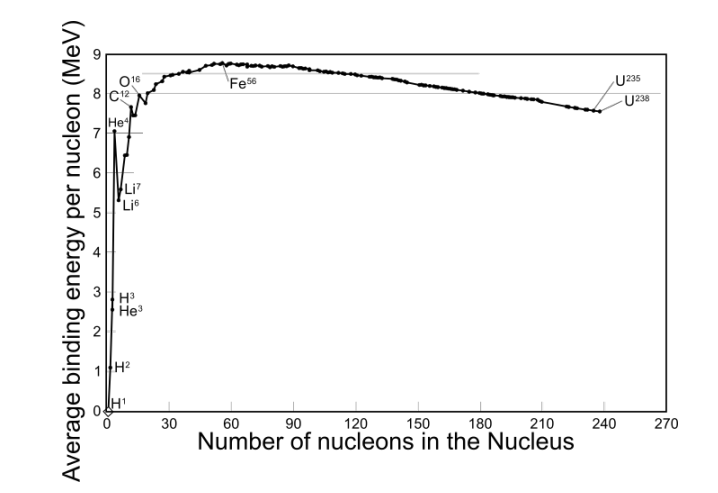
\includegraphics[width=0.8\linewidth]{images/BindingEnergyOfElements.png}
    \caption{Binding energy of the elements}
    \label{BindingEnergy}
\end{figure}

\begin{align}
\text{D}_1^2 +  \text{T}_1^3 &\to  \text{He}_2^4 + n_0^1 + 17.6 \, \rm{MeV} \\
\text{D}_1^2 +  \text{D}_1^2 &\to  \text{He}_2^3 + n_0^1 + 3.27 \, \rm{MeV}
\label{fusionreactions}
\end{align}

Its easy to prove, just by adding the masses of the reactants and compare with the products, we find that there is some mass missing, this mass corresponds with the energy mass relation $\Delta E = \Delta m c^2 = 17.6 \, \rm{MeV}$ describing the release of energy has to be in relation with the excess mass $\Delta m$ of each side of the equation. Said released energy is turned into net kinetic energy. Where the preferred reaction is that of Deuterium and Tritium due to their high cross section at lower energies compared with the second reaction and their derivatives. There is also a reaction between deuterium and helium-3 but its cross section is smaller than the previous.

\begin{figure}
    \centering
    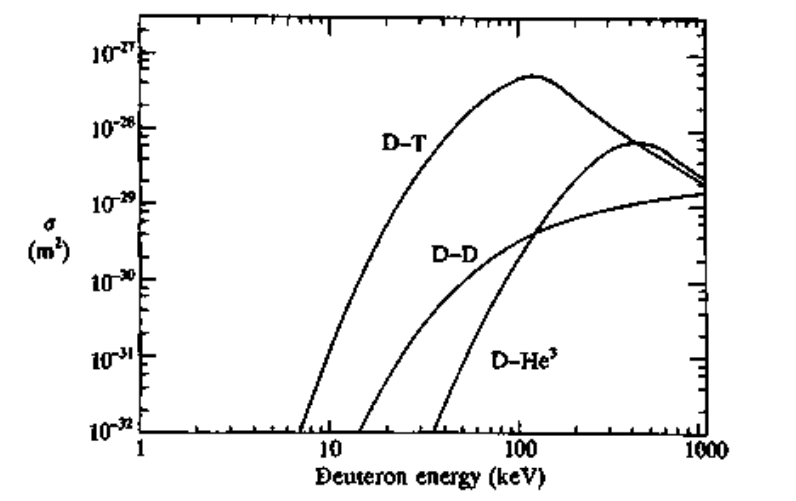
\includegraphics[width=0.8\linewidth]{images/DeuteronCrossSection.png}
    \caption{Deuteron cross section with $\ce{D}_1^2$, $\ce{T}_1^3$ and $\ce{He}_2^3$}
    \label{DeuteronCrossSection}
\end{figure}

This cross sections peak at energies that correspond with very high temperatures, this causes the gas to be fully ionized therefore resulting in neutral plasma. Material confinement cannot contain this temperatures, therefore another types of confinement must be used.

\subsection{Reaction rate}

Given the cross sections and a specific density, we should be able to tell how often this fusion events will take place. We calculate this. Assuming velocity distribution to be Maxwelian, $\vec{v}' = \vec{v}_1 - \vec{v}_2$ and the rate of reaction per unit volume is,

\begin{equation}
    \mathcal{R} = \int \int \sigma(v')v'f_1(\vec{v}_1)f_2(\vec{v}_2) d^3v_1d^3v_2
\end{equation}
Having that the reaction cross section has to be proportional to both the cross section and the relative velocity velocity, hence $\sigma(v') v'$.
Making sense of the equation, calculates the overlap of the distribution function across all possible velocities in the distribution and weights by the reaction cross section. \\

Calculate this explicitly \\


From this, the power generated will be proportional to both deuterium and tritium densities $n_T, n_D$, mean energy liberated per reaction $\epsilon$ and the reaction rate $\langle \sigma v\rangle$.

\begin{equation}
    P_{gen} = n_T n_D \langle \sigma v\rangle \epsilon
\end{equation}
which can be rewritten in term of total density

\begin{equation}
    P_{gen} = n_D(n - n_D) \langle \sigma v\rangle \epsilon
\end{equation}
which is maximized if the density $n_D \approx \frac{1}{2}n$

\begin{equation}
    P_{gen} = \frac{1}{4}n^2 \langle \sigma v\rangle \epsilon
\end{equation}
\subsubsection{Ignition and confinement time}

The total thermal energy will be consistent with the thermal energy of the electrons and ions, and since from previous results we now that we can maximize the power generated by having a plasma with $n_e = n_i = n$

\begin{equation}
    W = \int dV \left(\frac{3}{2}k_B T n_i\right) + \int dV \left(\frac{3}{2}k_B T n_e\right)
\end{equation}

\begin{equation*}
    W = \int dV k_B T n = 3k_B \langle n T \rangle
\end{equation*}
 with $\langle n T \rangle$ being the average value of the product

We define the energy lost in a period $\tau$ or energy confinement time as
\begin{equation}
    P_L = \frac{W}{\tau} \to  \tau = \frac{W}{P_L} 
\end{equation}
Where, to sustain the reaction the energy lost is replenished such that $P_H = P_L$

\begin{equation}
     \tau = \frac{W}{P_H} 
\end{equation}
where $\sim \frac{4}{5}$ of $P_{gen}$ are carried by the neutron and the rest by the $\alpha$-particle, given that it's almost 4 times easier to accelerate a neutron than a helium nucleus. Neutrons don't interact with the plasma, but alpha particles propagate following magnetic field lines, they are confined. This causes the $\alpha$-particle to have its own collision events at $3.5 \, \rm{MeV}$ with the plasma, heating it. The measure of this heating in a volume $V$ is,
\begin{equation}
    P_{\alpha} = \frac{1}{4}\int n^2\langle\sigma v\rangle \epsilon dV
\end{equation}
\begin{equation}
    P_{\alpha} = \frac{1}{4} \overline{n_{\alpha}^2  \langle \sigma v\rangle } \epsilon_{\alpha} V 
\end{equation}
This allows us to compare the power generated by fusion, the $\alpha$-particle heating and the thermal energy.
\begin{equation}
    P_{H} + P_{\alpha} = W
\end{equation}
The energy supplied to balance the energy lost by external heating and the $\alpha$-heating has to be equal to the total thermal energy of the plasma in a confinement time basis. 
\begin{equation}
    P_{H} + \frac{1}{4} \overline{n_{\alpha}^2  \langle \sigma v\rangle } \epsilon_{\alpha} V =  \frac{3k_B \langle n T \rangle}{\tau}V
\end{equation}
This external heat source can be achieved in many ways. Three main methods are used: neutral beam injection, ion cyclotron heating, and electron cyclotron heating.

The $\alpha$-particle collisions increasingly heat the confinement of D-T plasma. If the adequate confinement conditions are reached, the heating by $\alpha$-particles can overcome the energy losses and 

\begin{equation}
    P_{H} = \left( \frac{3k_B \langle n T \rangle}{\tau}- \frac{1}{4} n_{\alpha}^2  \langle \sigma v\rangle \epsilon_{\alpha} \right) V
\end{equation}

The condition for a self-sustaining reaction or "Ignition", is that $P_H=0$ (which means no external sources of heat).

\begin{equation}
    n_{\alpha}\tau >\frac{12 k_B \langle n T \rangle}{n_{\alpha}  \langle \sigma v\rangle \epsilon_{\alpha} } 
\end{equation}
For the densities being in the same order of magnitude, so we end up with the ignition condition
\begin{equation}
    n_{\alpha}\tau > 1.5 \times 10^{20} \, \rm{m}^{-3}\rm{s}
\end{equation}

But, instead of taking the value of temperature as a given for and substitute the reaction rate $\langle \sigma v\rangle \propto T^2 $ we get a more precise relation now with the triple product $n_{\alpha}\tau T$. We change notation to fit the book but lets take $k_BT \to T'$ and is now in keV.

\begin{equation}
    n\tau T' > 3 \times 10^{21} \, \rm{m}^{-3} \rm{keV} \, \rm{s}
\end{equation}

This is a very good criterion to obtain ignition. Some values that would be required to fulfill this condition are $n = 10^{20} \, \rm{m}^{-3}$, $T' = 10 \, \rm{keV}$ and $\tau = 3 \, \rm{s}$. Which is still difficult to obtain due to several instability, wall interactions and neutron feeding.

\begin{center}
\begin{tabular}{||c||c||c||}
\hline
\textbf{$T' = k_BT$} & \textbf{$\tau$} & \textbf{$n$} \\ \hline
   10 \, \rm{keV} & $3 \, \rm{sec}$  & $\sim 10^{20}$  \\ \hline
\end{tabular}
\end{center}
Important to remember that this calculation or condition, comes from taking into account $\alpha$-particle heating as one big contributor to keeping the reaction sustained. In the first versions of this condition, the Lawson criterion would only consider external heating sources and neglect alpha heating. He also considered bremsstrahlung which is a weak loss of energy in a tokamak plasma.

\begin{figure}[H]
    \centering
    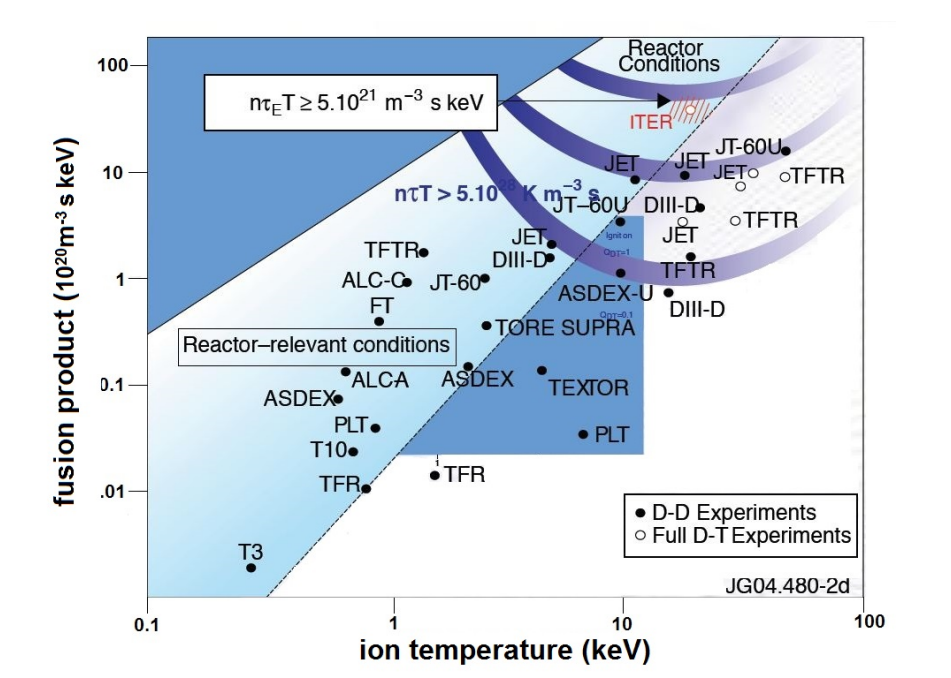
\includegraphics[width=0.8\linewidth]{images/TripleProductCriterion.png}
    \caption{Triple product criterion}
    \label{fig:enter-label}
\end{figure}

As a measure of sucess it the Q-factor, basicly the ratio of thermonuclear power generate/produced $P_{gen}$ and the heating power $P_H$.
\begin{equation}
    Q = \frac{P_{gen}}{P_{H}}
\end{equation}
But, it was discussed before that the Power generated by the reaction, was related to the $\alpha$-heating by a factor of 5. We can use this to our advantage, making it easier to measure.

\begin{equation}
    Q = \frac{5P_{\alpha}}{P_{H}}
\end{equation}

If ignition is obtained, then $P_H \to 0$ and $Q\to \infty$. So the goal is now to obtain a $Q=1$ corresponding with this $20\%$ power coming from $\alpha$-particles, which is at the very moment of ignition. 

Adding a time dependence to the relation between power supplied, thermal energy and $\alpha$-heating we can describe the way towards ignition.
Starting from,
\begin{equation}
     \frac{dE_{T}}{dt} = \frac{P_{H}}{V} + \frac{1}{4} n_{\alpha}^2  \langle \sigma v\rangle \epsilon_{\alpha} - \frac{3k_B \langle n T \rangle}{\tau}
\end{equation}
Where the right side corresponds with the rate of change of the total thermal energy in the system. The moment this energies balance corresponds to ignition, and the behaviour of this parameters has been discussed. Where as the temperature $T$ increases, the particles start to collide, which fires $\alpha$-heating and at some point it will replace $P_H$ as the supply for heat, so $P_H$ can be reduced only to provide for the energy losses.

The thermal energy $E_T$ can be expressed similarly to the plasma thermal energy $E_T = 3nk_BT$

\begin{equation}
    3nk_B \frac{dT}{dt} = \frac{P_{H}}{V} + \frac{1}{4} n_{\alpha}^2  \langle \sigma v\rangle \epsilon_{\alpha} - \frac{3k_B \langle n T \rangle}{\tau(n,T)}
\end{equation}

Then we consider the value of temperature and confinement time needed to achieve stability.
\begin{equation}
    3\frac{k_BT}{\tau} = 3\frac{T'}{\tau} = \frac{1}{4} n_{\alpha}  \langle \sigma v\rangle \epsilon_{\alpha}
    \label{weakeq}
\end{equation}
We are assume that this stability condition is independent of energy supplied, since we just balanced energy difference between thermal energy of plasma and $\alpha$-heating.

But we are interested in a more precise condition for the bounds ot $T, \tau$ that represent equilibrium. We assume a small change in temperature $\Delta T$ (assumed to be small) and expand $\langle \sigma v \rangle$ and $\tau$ to first order in terms of temperature. We adopt $T \to k_BT$ to follow the book \textit{Tokamaks by J. Wesson}.
Where the subscript $eq$ means evaluated at equilibrium position $T$.
\begin{align}
    \langle \sigma v \rangle &\approx \langle \sigma v \rangle_{eq} + \Delta T\frac{d\langle \sigma v \rangle}{dT} \\
    \tau &\approx \tau_{eq} + \Delta T\frac{d\tau}{dT}
\end{align}

We will need to consider the relaxation of the system, on other words, the heat evolution of the system.
\begin{equation}
    \frac{dT}{dt} = - \frac{T}{\tau}
\end{equation}
If we perturbe the system, will allows to simplify the expansion of $\tau$.
\begin{align}
    \frac{d(T+\Delta T)}{dt} &= - \frac{T+\Delta T} {\tau_{eq} } \left({1 + \frac{\Delta T}{\tau_{eq} }\frac{d\tau}{dT}} \right)^{-1} \\
    &\approx - \frac{T+\Delta T} {\tau_{eq} } \left(1 - \frac{\Delta T}{\tau_{eq}}\frac{d\tau}{dT}\right) \\
    &\approx - \frac{T+\Delta T} {\tau_{eq} } + \frac{T+\Delta T} {\tau_{eq} }\frac{\Delta T}{\tau_{eq}}\frac{d\tau}{dT})\\
    &\approx - \frac{T+\Delta T} {\tau_{eq} } + \frac{T\Delta T} {\tau_{eq}^2 }\frac{d\tau}{dT})
\end{align}

We notice that by getting $\frac{d\delta T}{dt}$ many terms will cancel and we will get
\begin{equation}
    3n \frac{d \Delta T}{d t} =
\left[-3n \left( \frac{1}{\tau_{eq}} - \frac{T}{\tau_{eq}^2} \frac{d \tau_{eq}}{d T} \right)
+ \frac{1}{4} n^2 \frac{d \langle \sigma v \rangle}{d T} \varepsilon_{\alpha} 
\right] \Delta T
\end{equation}

and substituting (\ref{weakeq}) in it for 

\begin{equation}
    3n \frac{d\Delta T}{dt} = \frac{1}{4} \pi^2 \langle \sigma v \rangle \frac{\xi_{\alpha}}{T} 
\left( -1 + \frac{T}{\tau_{eq}} \frac{d\tau_{eq}}{dT} + \frac{T}{\langle \sigma v \rangle} \frac{d\langle \sigma v \rangle}{dT} \right) \Delta T
\label{ETvariation}
\end{equation}

To have a failure at ignition due to temperature instabilities, then the right side of (\ref{ETvariation}) has to be negative.

\begin{equation}
 \frac{T}{\tau_{eq}} \frac{d\tau_{eq}}{dT}   < 1 - \frac{T}{\langle \sigma v \rangle} \frac{d\langle \sigma v \rangle}{dT}
\end{equation}
which is the strong form of the equlibrium condition
\section{Tokamaks}

A tokamak is a toroidal magnetic confinement system. The fusion devices using this systems where built in Russia in the 1950's. The proposal to use controlled thermonuclear fusion for industrial purposes and a specific scheme using thermal insulation of high-temperature plasma by an electric field was first formulated by the Soviet physicist Oleg Lavrentiev in a mid-1950 paper. In 1951, Andrei Sakharov and Igor Tamm modified the scheme by proposing a theoretical basis for a thermonuclear reactor, where the plasma would have the shape of a torus and be held by a magnetic field.

\subsection{Magnetic confinement}

The main magnetic field in the system is $B_{\phi}$ which points in the in the polar angle, here called \textit{Toroidal} by coils with external current.

\begin{figure}[H]
    \centering
    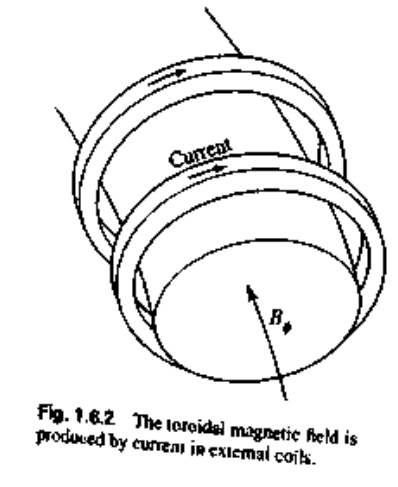
\includegraphics[width=0.5\linewidth]{images/ToroidalMagneticFieldCoils.png}
    \caption{Toroidal field (TF) coils (\textit{figure from Tokamak by J. Wesson})}
    \label{fig:enter-label}
\end{figure}

\begin{figure}[H]
    \centering
    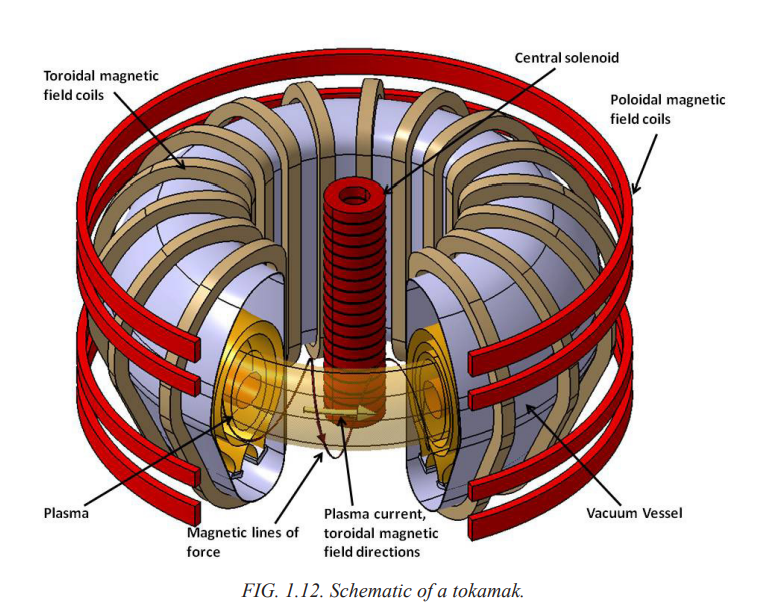
\includegraphics[width=0.5\linewidth]{images/TokamaksSchematic.png}
    \caption{Caption}
    \label{fig:enter-label}
\end{figure}

\subsection{Challenges}

Sputtering and tritium breeding
MHD instabilities
tungsten wall sputtering and photon emission (line emission cooling)
berilyum wall

\subsection{Instabilities}

Vertical displacements events (VDE)

\section{Stellarator}

\subsection{Magnetic confinement}

\subsection{Challenges}

\subsection{Instabilities}

\newpage

%\begin{acknowledgements}
%If you'd like to thank anyone, place your comments here
%and remove the percent signs.
%\end{acknowledgements}

% BibTeX users please use one of
%\bibliographystyle{spbasic}      % basic style, author-year citations
%\bibliographystyle{spmpsci}      % mathematics and physical sciences
%\bibliographystyle{spphys}       % APS-like style for physics
%\bibliography{}   % name your BibTeX data base

% Non-BibTeX users please use
\begin{thebibliography}{}
%
% and use \bibitem to create references. Consult the Instructions
% for authors for reference list style.
%
\bibitem{RefJ}
% Format for Journal Reference
Wesson, J. and Campbell, D. Tokamaks. International series of monograms (OUP
Oxford, 2011). ISBN 978-0-19-959223-4.
\bibitem{RefB}
 Chen, F. F. Introduction to Plasma Physics and Controlled Fusion (Springer International Publishing, Cham, 2016). ISBN 978-3-319-22308-7 978-3-319-22309-4.
\bibitem{refN}
Schwarz, N. (2020). Vertical Displacement Events in ASDEX Upgrade (IPP 2020-14). Max Planck Institute for Plasma Physics (IPP Garching).
\end{thebibliography}

\end{document}
% end of file template.tex

